Simulacemi zjistěte tyto parametry tranzistorů NMOS a PMOS:

\begin{enumerate}
    \item {\bf Navrhněte kaskodové proudové zrcadlo na výstupu proudové reference podle obr. \ref{fig:sch_zadani}. (schéma z LTspice je součástí zadání)}
    \begin{figure}[h]
        \centering
        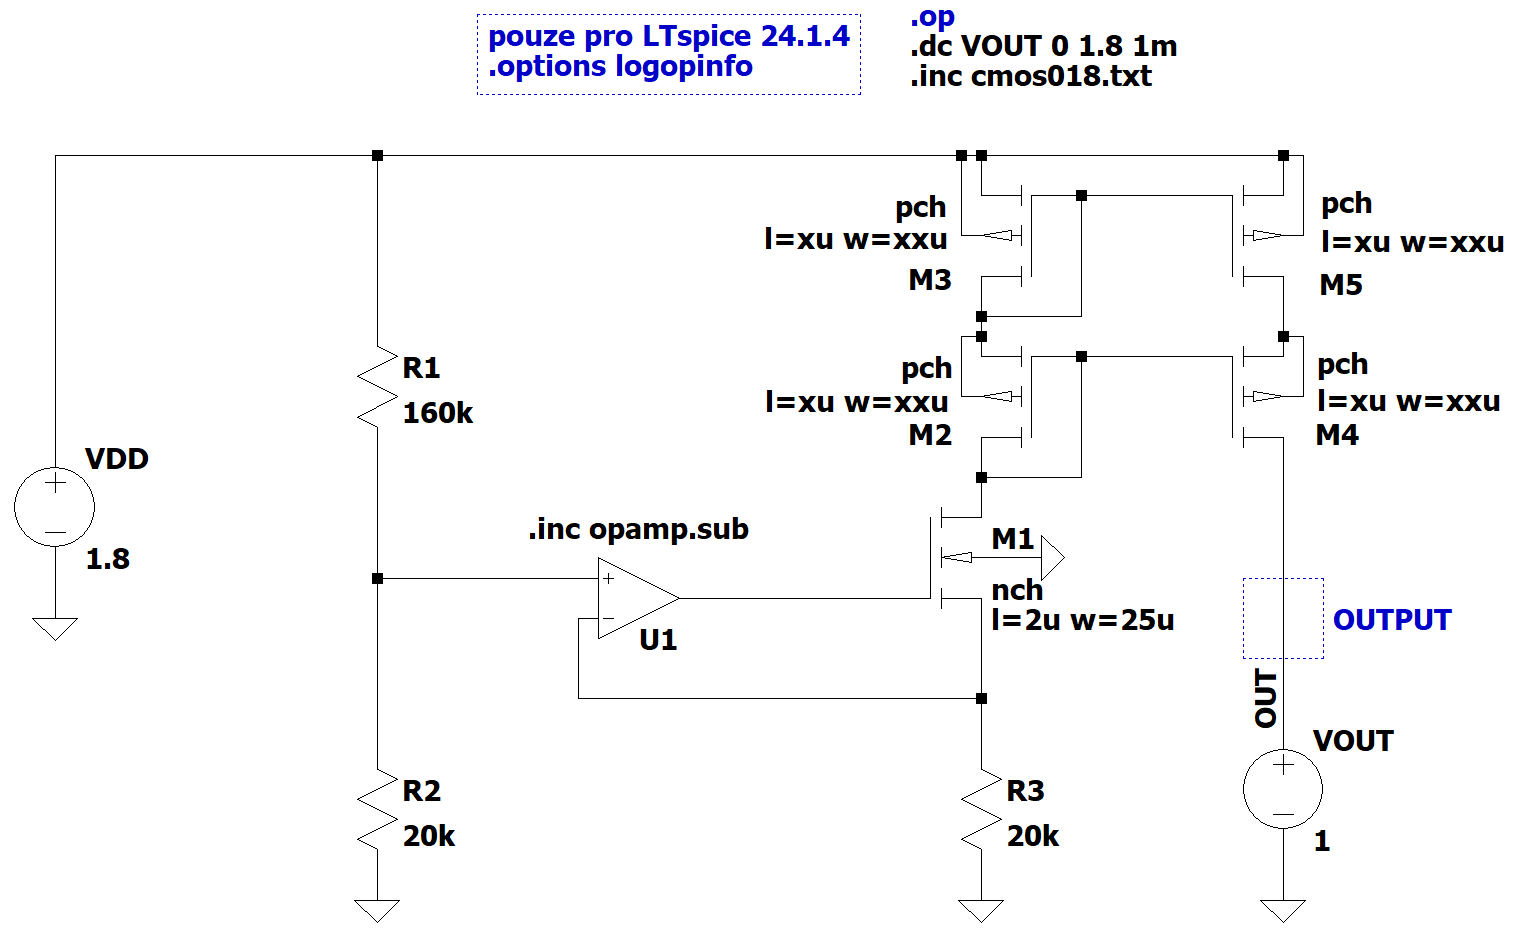
\includegraphics[height=0.3\textheight]{text/img/zadani.png}
        \caption{\label{fig:sch_zadani} Proudový zdroj s kaskádovým PZ}
    \end{figure}
    \begin{enumerate}
        \item Vypočítejte rozměry tranzistorů M2 - M5, výstupní odpor a výstupní rozsah proudového zrcadla (\textcolor{red}{P - výpočty ve formátu obecná rovnice, dosazení, výsledek}).
        \item Ověřte správný výpočet pomocí simulace .op (\textcolor{red}{P - schéma se zvýrazněnými U/I dle předlohy + printscreen pracovních bodů M2-M5 ze Spice Output Log})
        \item Simulací .dc zjistěte výstupní odpor a ověřte výstupní rozsah (\textcolor{red}{P - křivka s kurzory + viditelnou tabulkou pozic kurzorů})
    \end{enumerate}
    \item {\bf Navrhněte (popř. modifikované) Wilsonovo proudové zrcadlo s tranzistory NMOS s výstupním proudem \(20 \mu A\). Vstupní je \(10\mu A\).}
    \begin{itemize}
        \item Vypočítejte parametry všech součástek, výstupní odpor a výstupní rozsah proudového zrcadla (\textcolor{red}{P - výpočty ve formátu obecná rovnice, dosazení, výsledek}).
        \item Ověřte správný výpočet pomocí simulace .op (\textcolor{red}{P - schéma se zvýrazněnými U/I + printscreen pracovní bodů tranzistorů ze Spice Output Log})
        \item Simulací .dc zjistěte výstupní odpor a ověřte výstupní rozsah (\textcolor{red}{P - křivka s kurzory + viditelnou tabulkou pozic kurzorů})
    \end{itemize}
\end{enumerate}
